\chapter{Quality of Service: Part 2}\label{quality-of-service-part-2}

\section{Classification / Marking}\label{classification-marking}

\begin{itemize}
\tightlist
\item
  The purpose of QoS is to give certain kinds of NETWORK TRAFFIC
  priority over other during congestion
\item
  CLASSIFICATION organizes network TRAFFIC (PACKETS) into TRAFFIC
  CLASSES (CATEGORIES)
\item
  CLASSIFICATION is fundamental to QoS.

  \begin{itemize}
  \tightlist
  \item
    To give PRIORITY to certain types of TRAFFIC, you have to IDENTIFY
    which types of TRAFFIC to give PRIORITY to.
  \end{itemize}
\item
  There are MANY methods of CLASSIFYING TRAFFIC

  \begin{itemize}
  \tightlist
  \item
    An ACL : TRAFFIC which is permitted by the ACL will be given certain
    TREATMENT, other TRAFFIC will not
  \item
    NBAR (Network Based Application Recognition) performs a \emph{DEEP
    PACKET INSPECTION,} looking beyond the LAYER 3 and LAYER 4
    information up to LAYER 7 to identify the specific kinds of TRAFFIC
  \item
    In the LAYER 2 and LAYER 3 HEADERS there are specific FIELDS used
    for this purpose
  \end{itemize}
\item
  The PCP (PRIORITY CODE POINT) FIELD of the 802.1Q Tag (in the ETHERNET
  HEADER) can be used to identify HIGH / LOW PRIORITY TRAFFIC

  \begin{itemize}
  \tightlist
  \item
    ** ONLY when there is a dot1q tag!
  \end{itemize}
\item
  The DSCP (DIFFERENTIATED SERVICES CODE POINT) FIELD of the IP HEADER
  can also be used to identify HIGH / LOW PRIORITY TRAFFIC
\end{itemize}

PCP / CoS

\begin{figure}
\centering
\pandocbounded{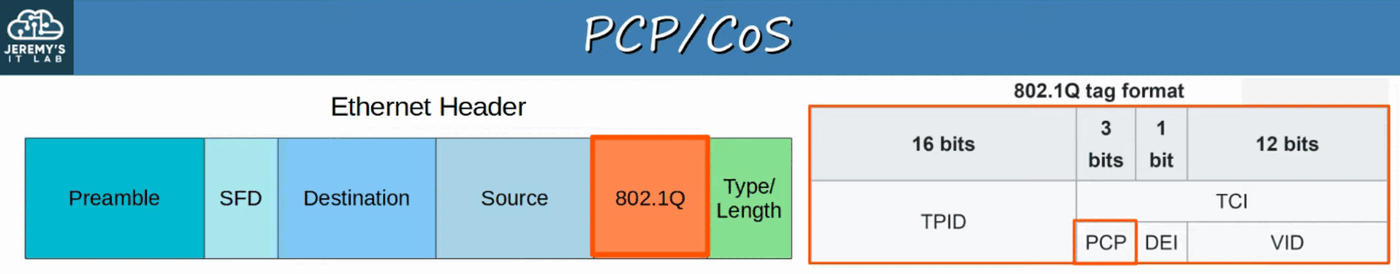
\includegraphics[keepaspectratio,alt={image}]{images/48-qos-quality-of-service/img-001.png}}
\end{figure}

\begin{itemize}
\tightlist
\item
  PCP is also known as CoS (CLASS OF SERVICE)
\item
  It's use is defined by IEEE 802.1p
\item
  3 bits = 8 possible values (2\^{}3 = 8)
\end{itemize}

\begin{figure}
\centering
\pandocbounded{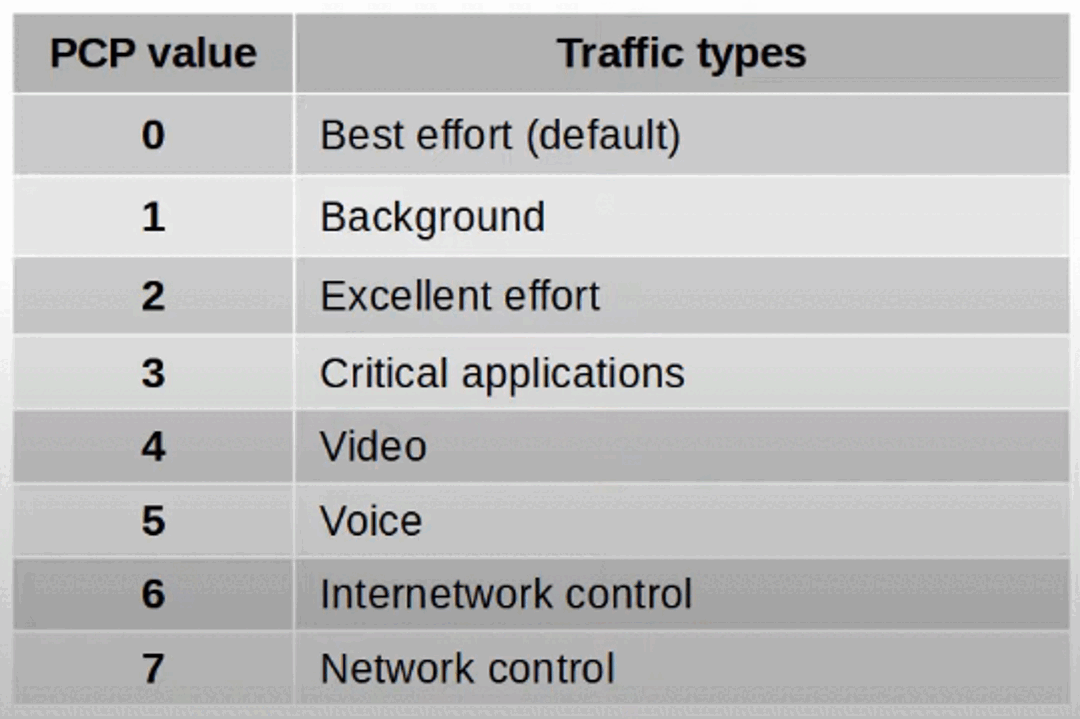
\includegraphics[keepaspectratio,alt={image}]{images/48-qos-quality-of-service/img-002.png}}
\end{figure}

\begin{itemize}
\tightlist
\item
  PCP VALUE 0:

  \begin{itemize}
  \tightlist
  \item
    ``BEST EFFORT'' DELIVERY means there is no guarantee that data is
    delivered or that it meets ANY QoS Standard. This is REGULAR TRAFFIC
    - NOT HIGH PRIORITY
  \end{itemize}
\item
  PCP VALUE 3 and 5:

  \begin{itemize}
  \tightlist
  \item
    IP PHONES MARK call signaling TRAFFIC (used to establish calls) as
    PCP3

    \begin{itemize}
    \tightlist
    \item
      They MARK the actual VOICE TRAFFIC as PCP5
    \end{itemize}
  \end{itemize}
\item
  Because PCP is found in the dot1q header, it can only be used over the
  following connections:

  \begin{itemize}
  \tightlist
  \item
    TRUNK LINKS
  \item
    ACCESS LINKS with a VOICE VLAN
  \end{itemize}
\item
  In the diagram below, TRAFFIC between R1 and R2, or between R2 and
  EXTERNAL DESTINATIONS will not have a dot1q tag. So, traffic over
  those links PCP cannot be marked with a PCP value.
\end{itemize}

\begin{figure}
\centering
\pandocbounded{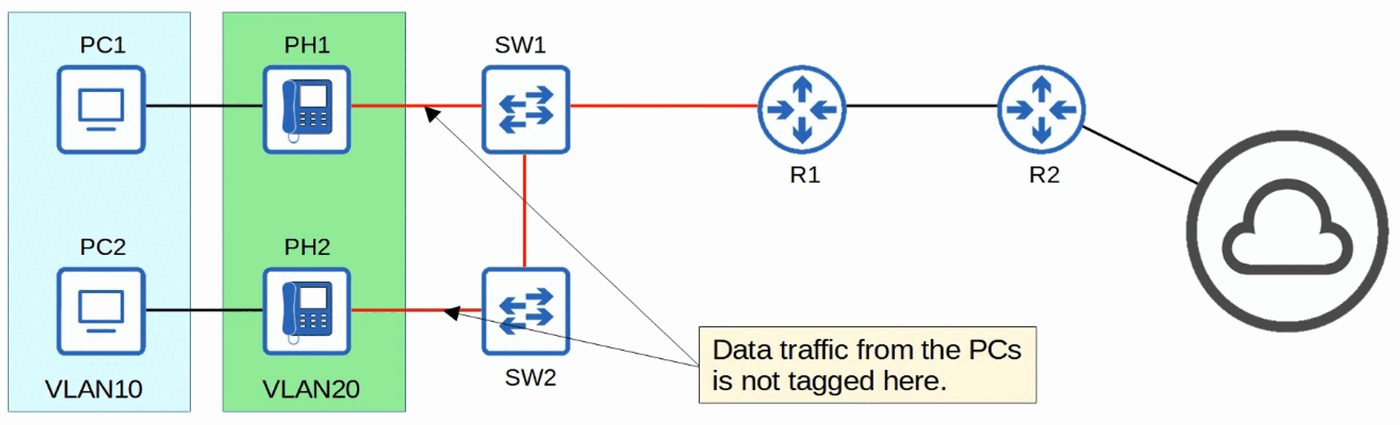
\includegraphics[keepaspectratio,alt={image}]{images/48-qos-quality-of-service/img-003.png}}
\end{figure}

THE IP ToS BYTE

\begin{figure}
\centering
\pandocbounded{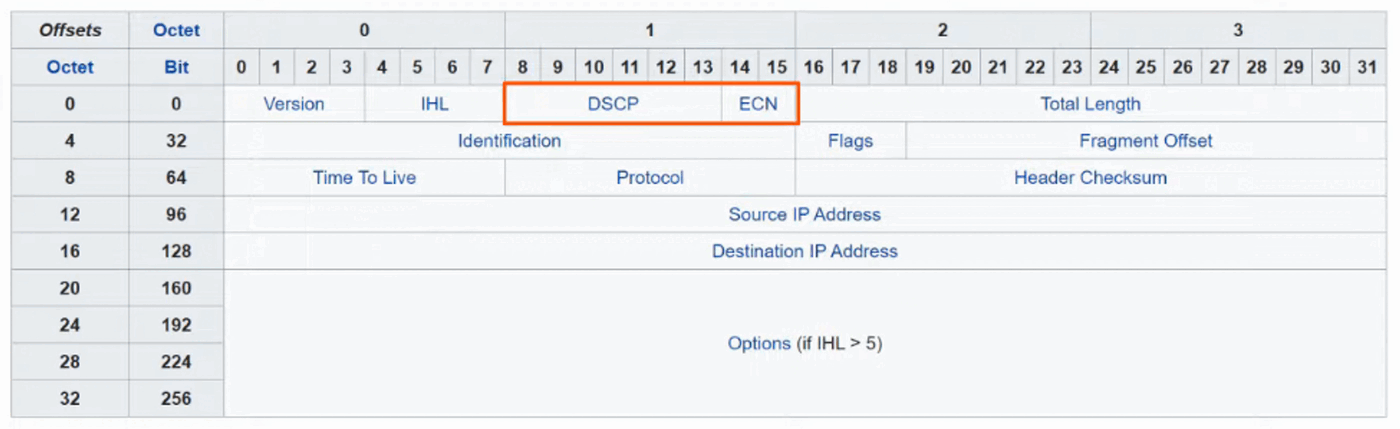
\includegraphics[keepaspectratio,alt={image}]{images/48-qos-quality-of-service/img-004.png}}
\end{figure}

\begin{figure}
\centering
\pandocbounded{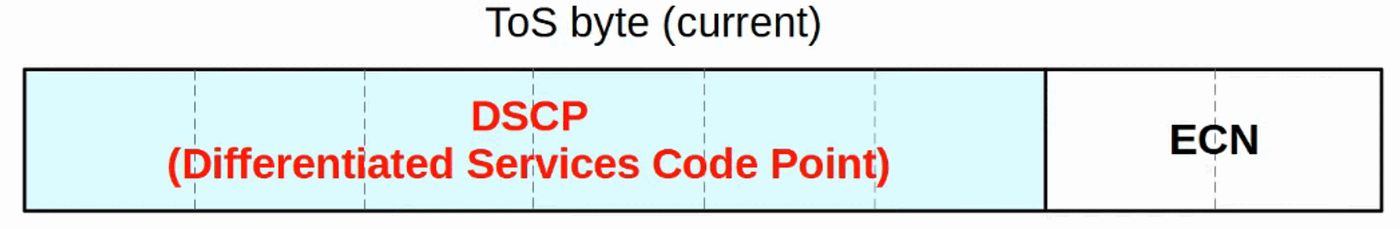
\includegraphics[keepaspectratio,alt={image}]{images/48-qos-quality-of-service/img-005.png}}
\end{figure}

(6 bits for DSCP and 2 bits for ECN)

\section{IP Precedence (Old)}\label{ip-precedence-old}

\begin{figure}
\centering
\pandocbounded{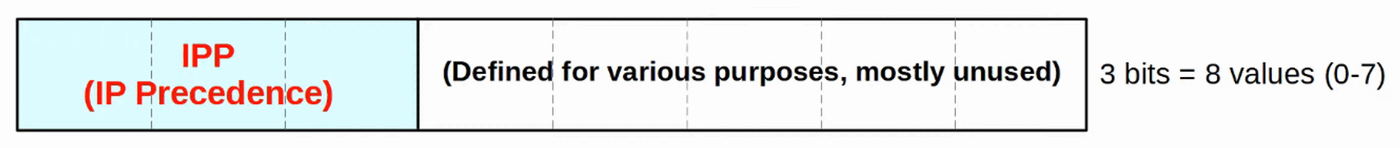
\includegraphics[keepaspectratio,alt={image}]{images/48-qos-quality-of-service/img-006.png}}
\end{figure}

\begin{itemize}
\tightlist
\item
  Standard IPP markings are similar to PCP:

  \begin{itemize}
  \tightlist
  \item
    6 and 7 are reserved to `network control traffic' (ie: OSPF Messages
    between ROUTERS)
  \item
    5 = VOICE
  \item
    4 = VIDEO
  \item
    3 = VOICE SIGNALLING
  \item
    0 = BEST EFFORT
  \end{itemize}
\item
  With 6 and 7 reserved, 6 possible values remain
\item
  Although 6 values is sufficient for many NETWORKS, the QoS
  REQUIREMENTS of some NETWORKS demand more flexibility
\end{itemize}

\section{DSCP (Current)}\label{dscp-current}

\begin{figure}
\centering
\pandocbounded{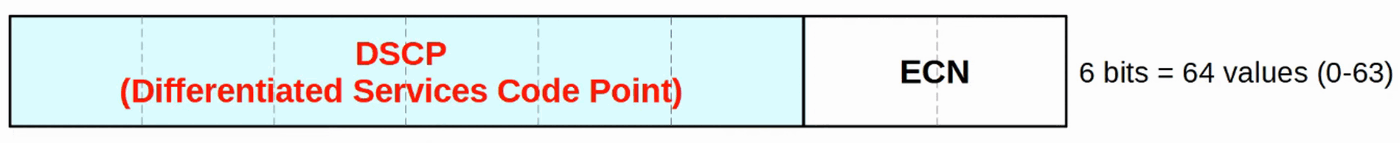
\includegraphics[keepaspectratio,alt={image}]{images/48-qos-quality-of-service/img-007.png}}
\end{figure}

\begin{itemize}
\tightlist
\item
  RFC 2474 (1998) defines the DSCP field, and other `DiffServ' RFCs
  elaborate on its use
\item
  With IPP updated to DSCP, new STANDARD MARKINGS had to be decided on

  \begin{itemize}
  \tightlist
  \item
    By having generally agreed upon STANDARD MARKINGS for DIFFERENT
    KINDS of TRAFFIC:

    \begin{itemize}
    \tightlist
    \item
      QoS DESIGN and IMPLEMENTATION is simplified.
    \item
      QoS works better between ISPs and ENTERPRISES
    \item
      etc.
    \end{itemize}
  \end{itemize}
\item
  You should be AWARE of the FOLLOWING STANDARD MARKINGS:

  \begin{itemize}
  \tightlist
  \item
    DEFAULT FORWARDING (DF) - Best Effort TRAFFIC
  \item
    EXPEDITED FORWARDING (EF) - Low Loss / Latency / Jitter TRAFFIC
    (usually voice)
  \item
    ASSURED FORWARDING (AF) - A set of 12 STANDARD VALUES
  \item
    CLASS SELECTOR (CS) - A set of 8 STANDARD VALUES, provides backward
    compatibility with IPP
  \end{itemize}
\end{itemize}

\section{DF / EF}\label{df-ef}

\section{Default Forwarding (DF)}\label{default-forwarding-df}

\begin{figure}
\centering
\pandocbounded{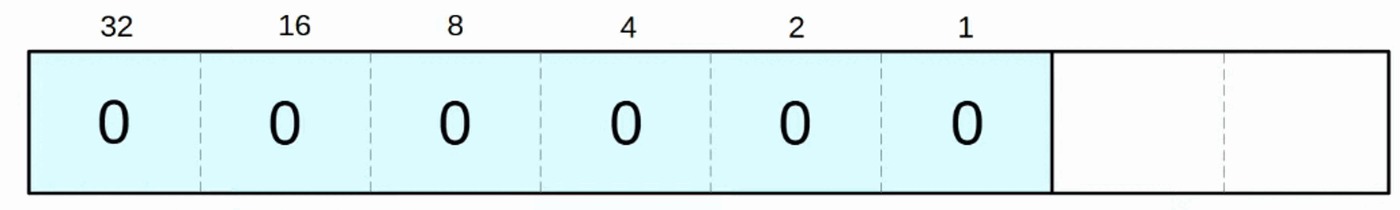
\includegraphics[keepaspectratio,alt={image}]{images/48-qos-quality-of-service/img-008.png}}
\end{figure}

\begin{itemize}
\tightlist
\item
  Used for BEST EFFORT TRAFFIC
\item
  The DSCP marking for DF is 0
\end{itemize}

\section{Expedited Forwarding (EF)}\label{expedited-forwarding-ef}

\begin{figure}
\centering
\pandocbounded{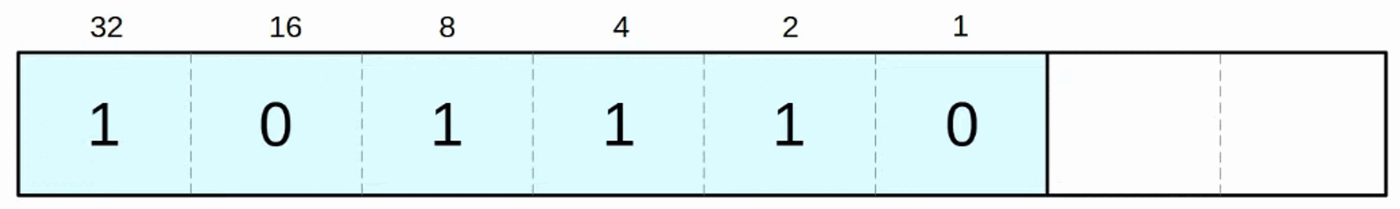
\includegraphics[keepaspectratio,alt={image}]{images/48-qos-quality-of-service/img-009.png}}
\end{figure}

\begin{itemize}
\tightlist
\item
  EF is used for TRAFFIC that requires Low Loss / Latency / Jitter
\item
  The DSCP marking for EF is 46
\end{itemize}

\section{Assured Forwarding (AF)}\label{assured-forwarding-af}

\begin{itemize}
\tightlist
\item
  Defines FOUR TRAFFIC CLASSES
\item
  ALL PACKETS in a CLASS have the same PRIORITY
\item
  Within each CLASS, there are THREE LEVELS of DROP PRECEDENCE

  \begin{itemize}
  \tightlist
  \item
    HIGHER DROP PRECEDENCE = More likely to DROP the PACKET during
    CONGESTION
  \end{itemize}
\end{itemize}

\begin{figure}
\centering
\pandocbounded{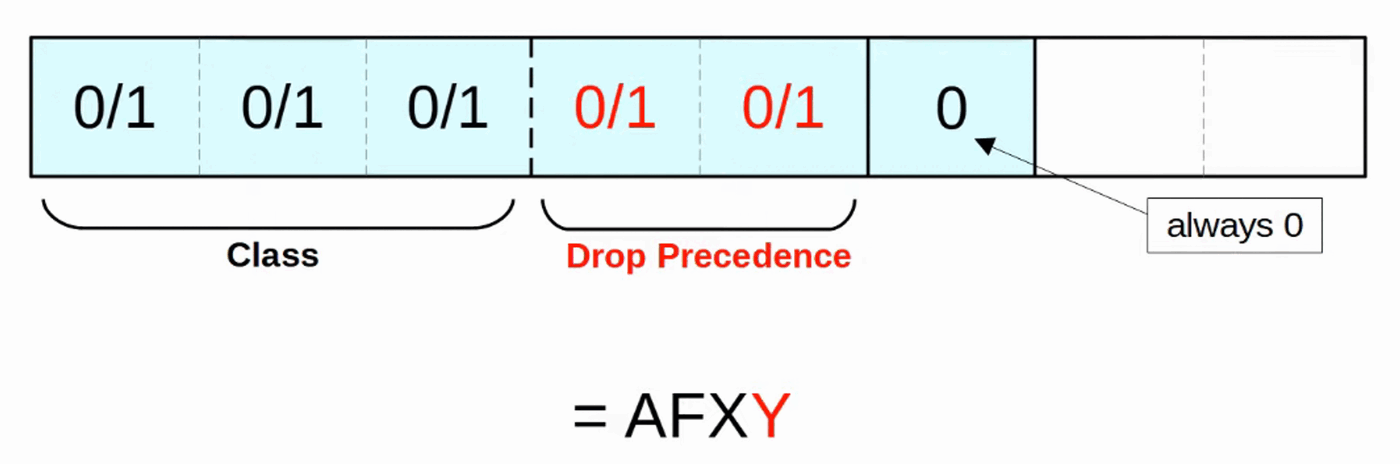
\includegraphics[keepaspectratio,alt={image}]{images/48-qos-quality-of-service/img-010.png}}
\end{figure}

\section{Examples}\label{examples}

\begin{figure}
\centering
\pandocbounded{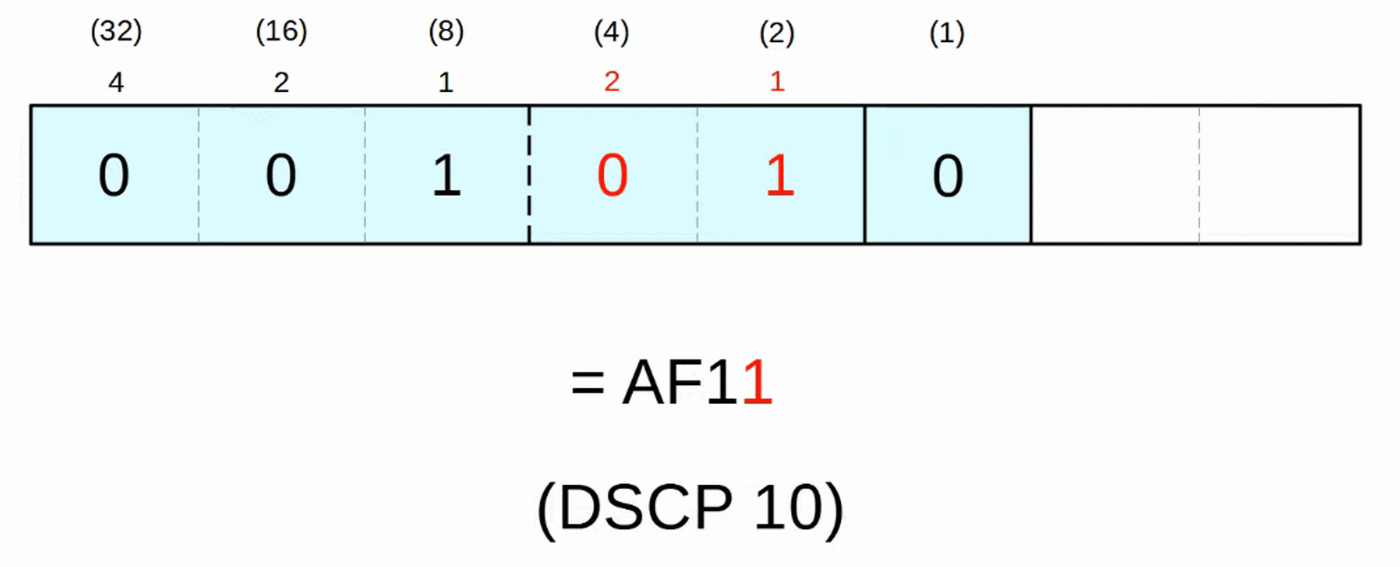
\includegraphics[keepaspectratio,alt={image}]{images/48-qos-quality-of-service/img-011.png}}
\end{figure}

\begin{figure}
\centering
\pandocbounded{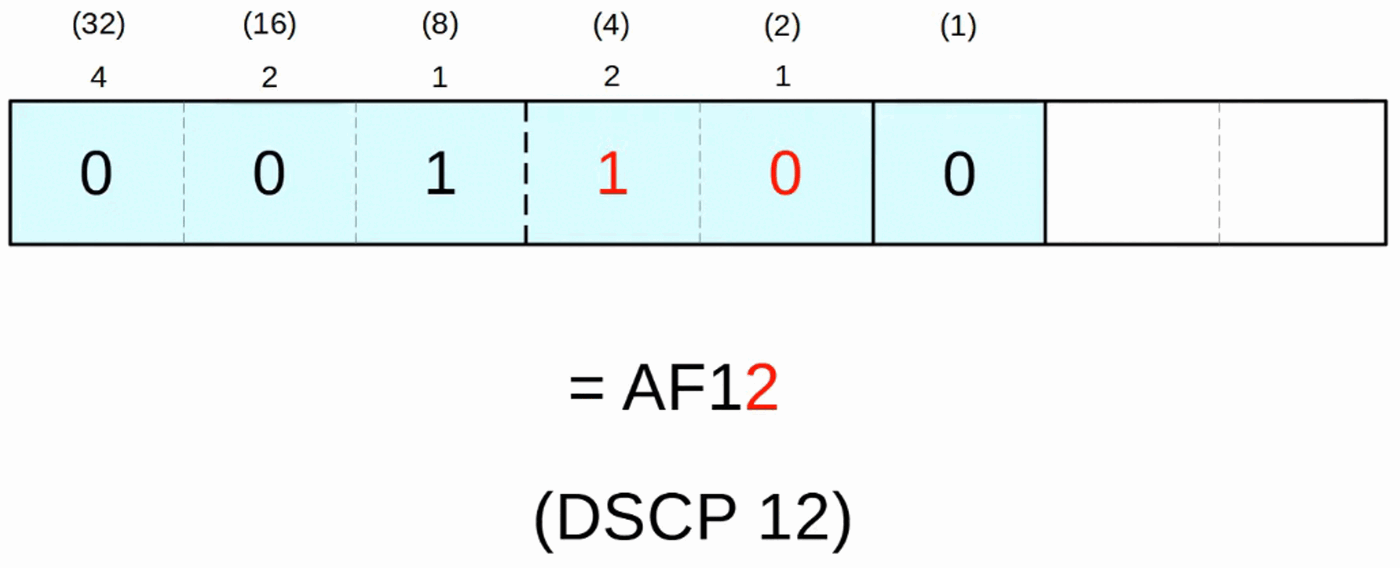
\includegraphics[keepaspectratio,alt={image}]{images/48-qos-quality-of-service/img-012.png}}
\end{figure}

\begin{figure}
\centering
\pandocbounded{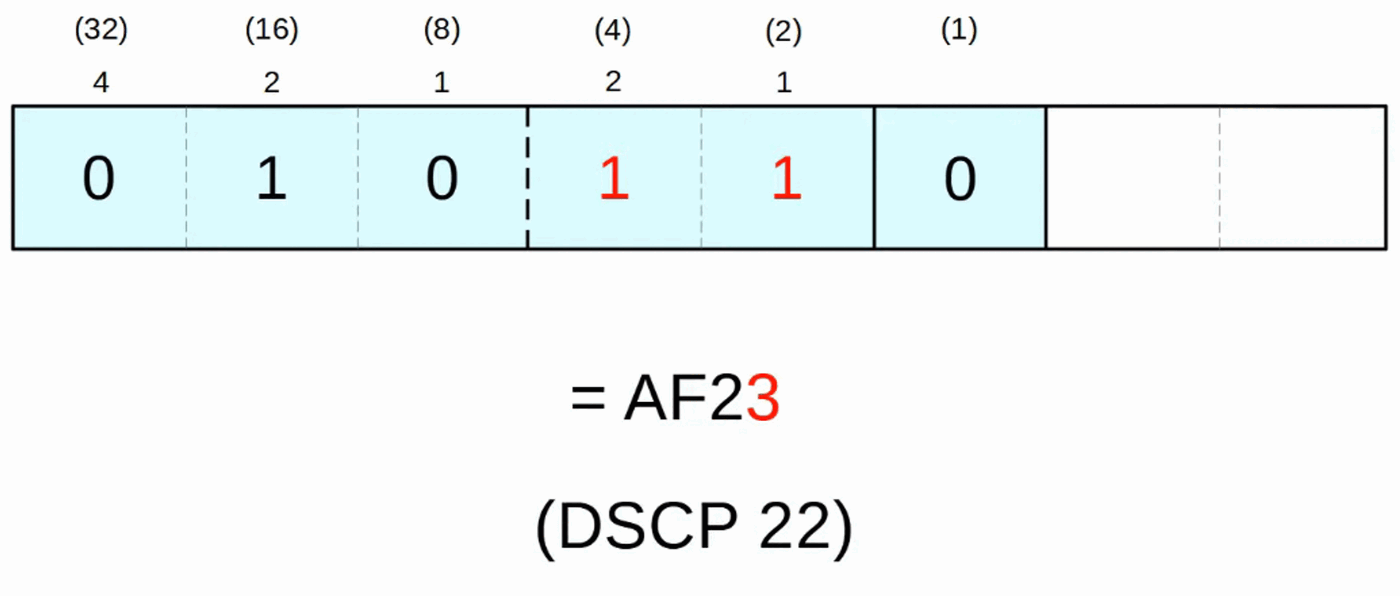
\includegraphics[keepaspectratio,alt={image}]{images/48-qos-quality-of-service/img-013.png}}
\end{figure}

\begin{figure}
\centering
\pandocbounded{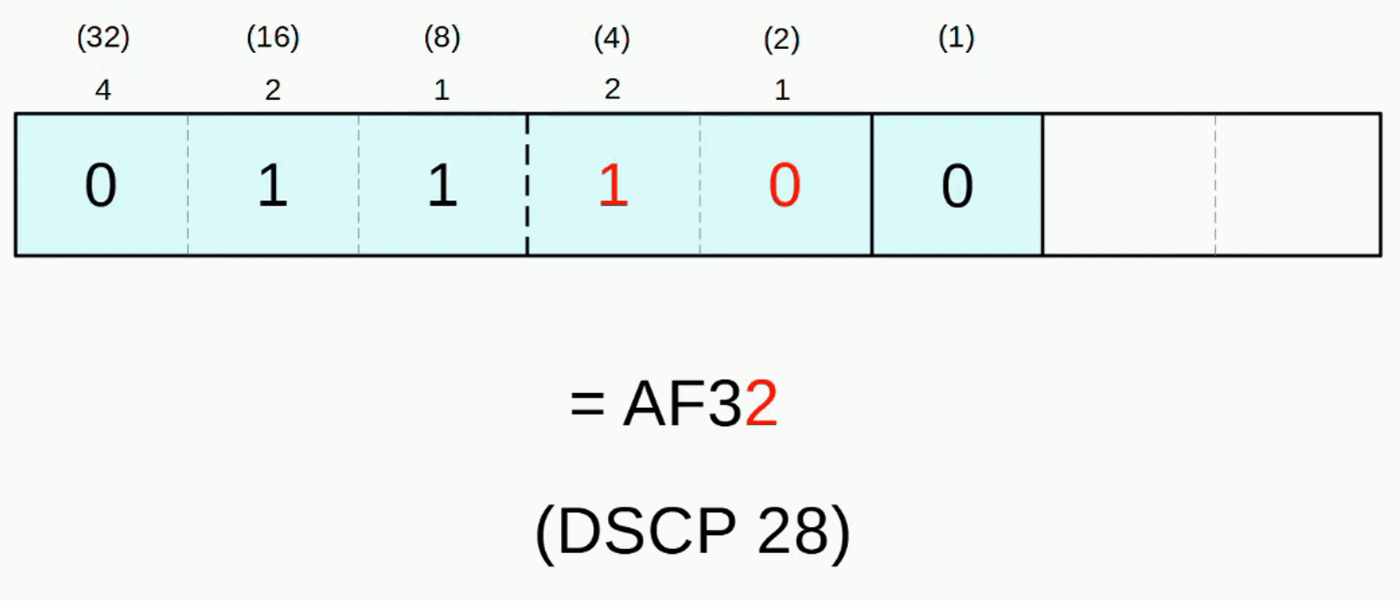
\includegraphics[keepaspectratio,alt={image}]{images/48-qos-quality-of-service/img-014.png}}
\end{figure}

\begin{figure}
\centering
\pandocbounded{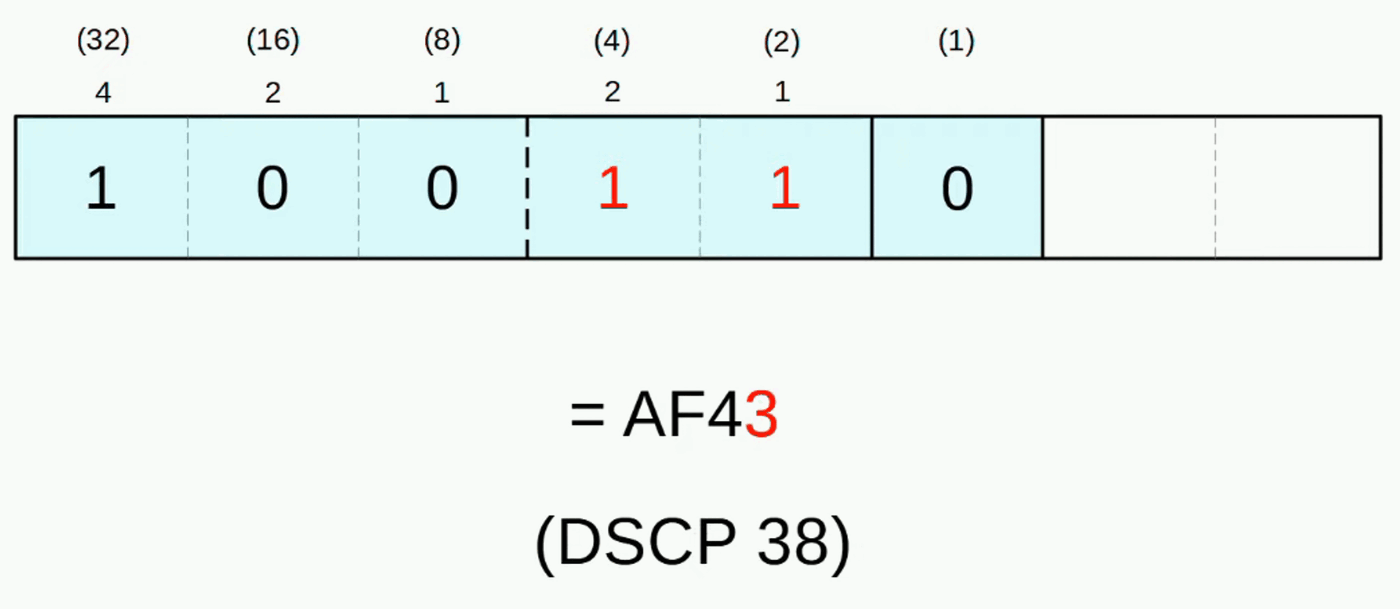
\includegraphics[keepaspectratio,alt={image}]{images/48-qos-quality-of-service/img-015.png}}
\end{figure}

\begin{figure}
\centering
\pandocbounded{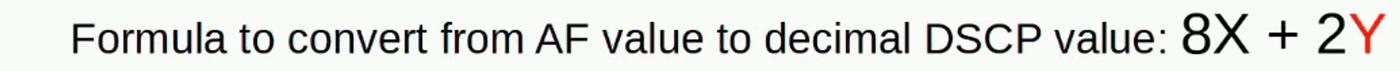
\includegraphics[keepaspectratio,alt={image}]{images/48-qos-quality-of-service/img-016.png}}
\end{figure}

\begin{figure}
\centering
\pandocbounded{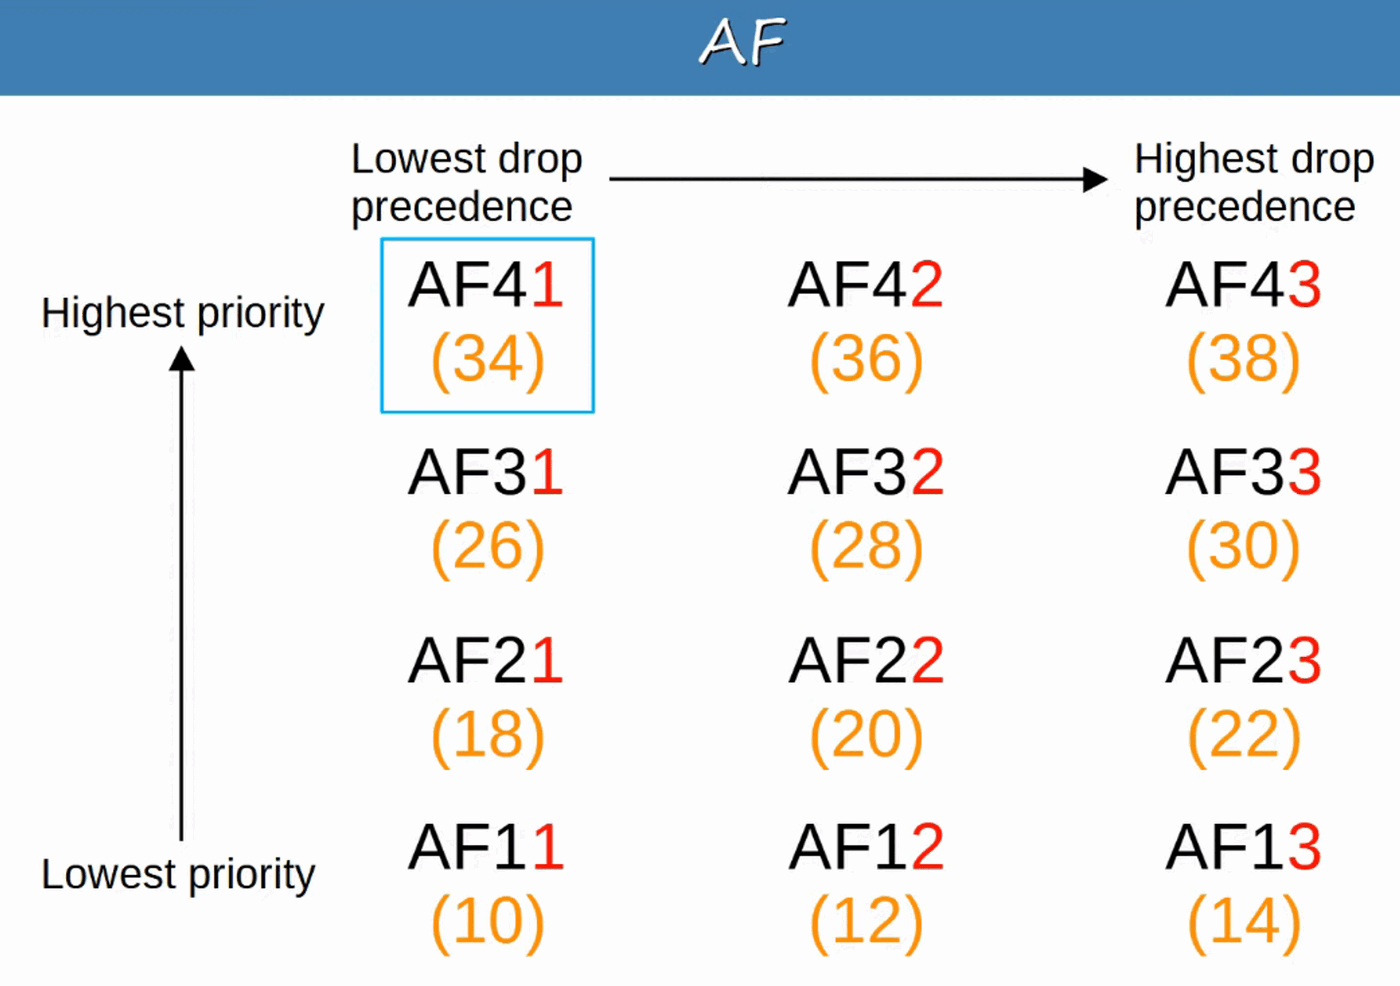
\includegraphics[keepaspectratio,alt={image}]{images/48-qos-quality-of-service/img-017.png}}
\end{figure}

\begin{itemize}
\tightlist
\item
  AF41 gets the BEST TREATMENT (Highest Priority / Lowest Drop)
\item
  AF13 gets the WORST TREATMENT (Lowest Priority / Highest Drop)
\end{itemize}

\section{Class Selector (CS)}\label{class-selector-cs}

\begin{itemize}
\tightlist
\item
  Defines EIGHT DSCP values for backward compatibility with IPP
\item
  The THREE BITS that were added for DSCP are set to 0, and the original
  IPP bits are used to make 8 values
\end{itemize}

\begin{figure}
\centering
\pandocbounded{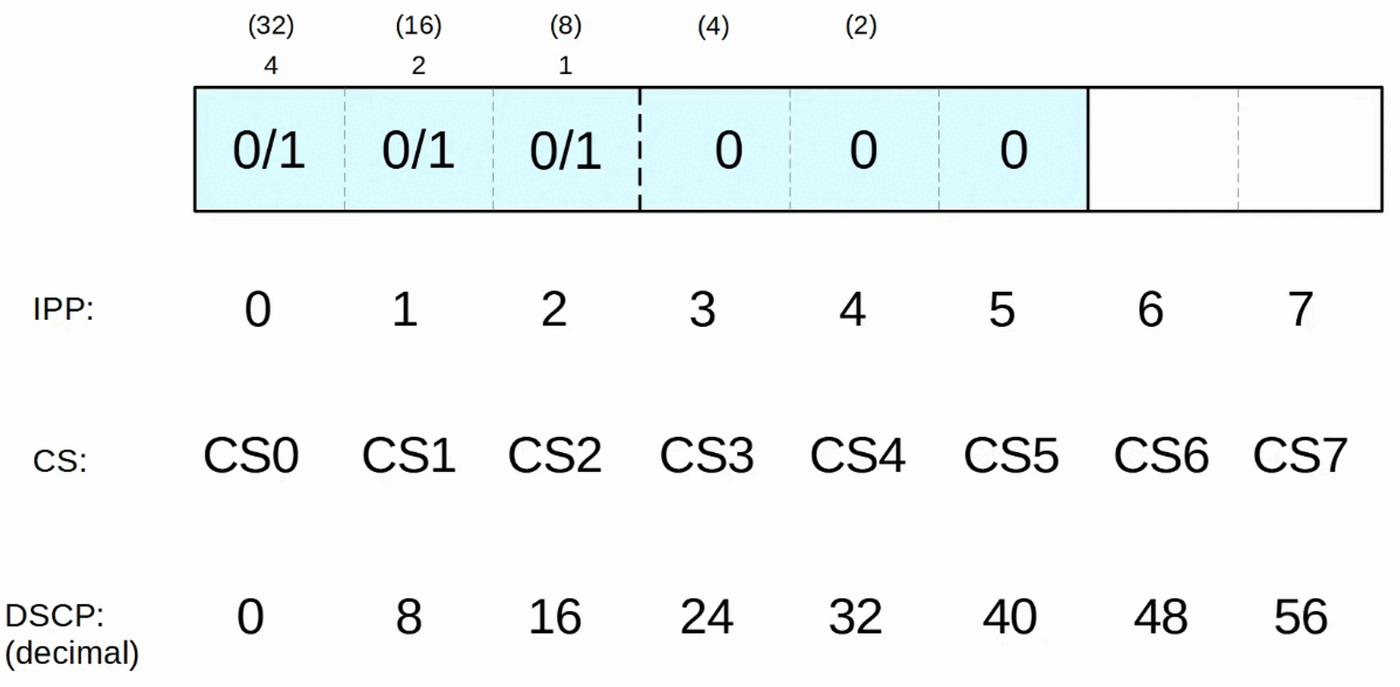
\includegraphics[keepaspectratio,alt={image}]{images/48-qos-quality-of-service/img-018.png}}
\end{figure}

\section{RFC 4954}\label{rfc-4954}

\begin{itemize}
\item
  RFC 4954 was developed with help of Cisco to bring ALL of these VALUES
  together and STANDARDIZE their use
\item
  The RFC offers MANY specific recommendations, but here are a few KEY
  ones:

  \begin{itemize}
  \tightlist
  \item
    VOICE TRAFFIC : EF
  \item
    INTERACTIVE VIDEO : AF4x
  \item
    STREAMING VIDEO : AF3x
  \item
    HIGH PRIORITY DATA : AF2x
  \item
    BEST EFFORT : DF
  \end{itemize}
\end{itemize}

\section{Trust Boundaries}\label{trust-boundaries}

\begin{itemize}
\tightlist
\item
  The TRUST BOUNDARY of a NETWORK defines where the DEVICE TRUST / DON'T
  TRUST the QoS MARKINGS of received messages
\item
  If the MARKINGS are TRUSTED:

  \begin{itemize}
  \tightlist
  \item
    DEVICE will forward the message without changing the MARKINGS
  \end{itemize}
\item
  If the MARKINGS are NOT TRUSTED:

  \begin{itemize}
  \tightlist
  \item
    DEVICE will change the MARKINGS according to configured POLICY
  \end{itemize}
\end{itemize}

\begin{figure}
\centering
\pandocbounded{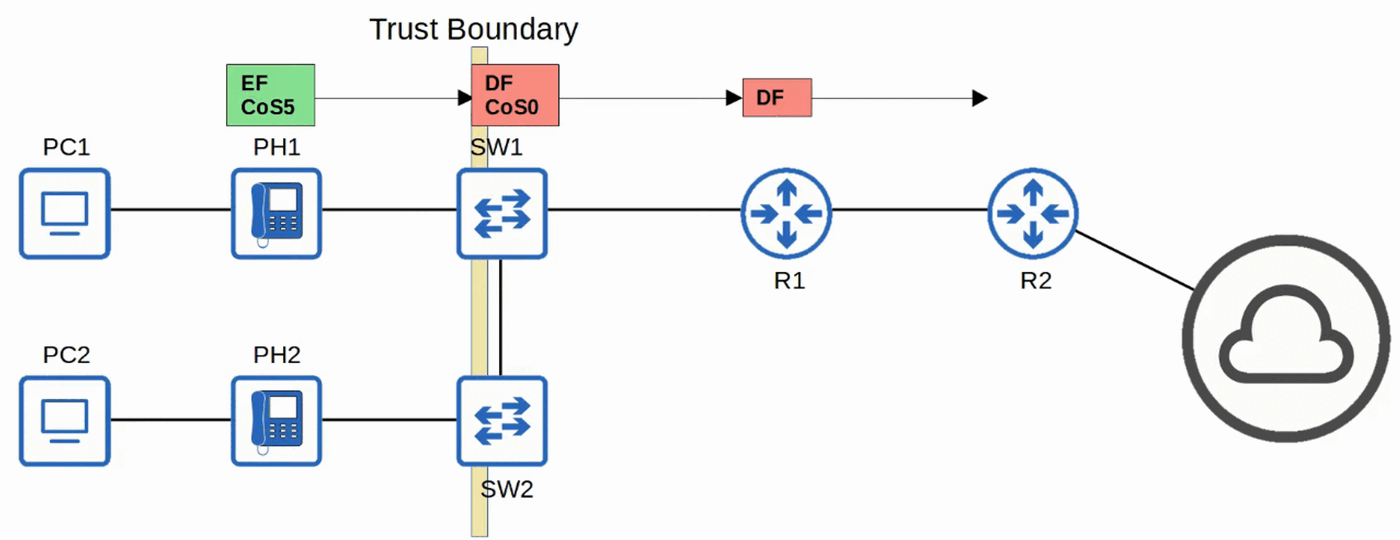
\includegraphics[keepaspectratio,alt={image}]{images/48-qos-quality-of-service/img-019.png}}
\end{figure}

\begin{itemize}
\tightlist
\item
  If an IP PHONE is connected to the SWITCH PORT, it is RECOMMENDED to
  move the TRUST BOUNDARY to the IP PHONES
\item
  This is done via CONFIGURATION on the SWITCH PORT connected to the IP
  PHONE
\item
  If a user MARKS their PC's TRAFFIC with a HIGH PRIORITY, the MARKING
  will be CHANGED (not trusted)
\end{itemize}

\begin{figure}
\centering
\pandocbounded{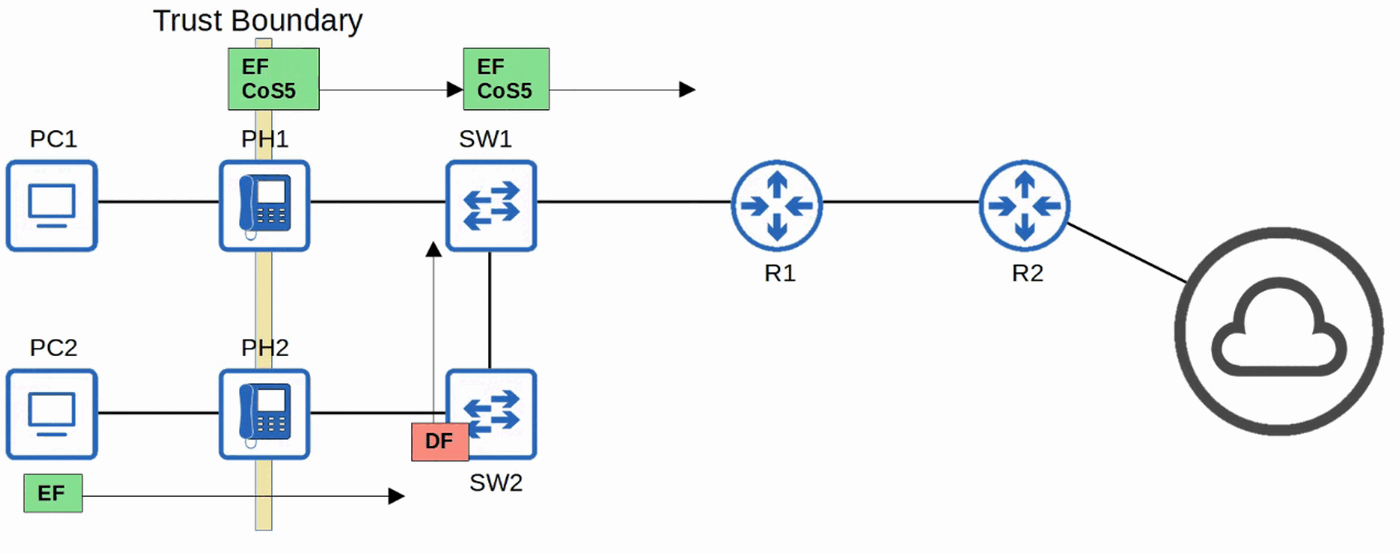
\includegraphics[keepaspectratio,alt={image}]{images/48-qos-quality-of-service/img-020.png}}
\end{figure}

\section{Queuing / Congestion
Management}\label{queuing-congestion-management}

\begin{itemize}
\tightlist
\item
  When a NETWORK DEVICE receives TRAFFIC at a FASTER PACE than it can
  FORWARD out of the appropriate INTERACE, PACKETS are placed in that
  INTERFACE'S QUEUE as they wait to be FORWARDED
\item
  When a QUEUE becomes FULL, PACKETS that don't FIT in the QUEUE are
  dropped (Tail Drop)
\item
  RED and WRED DROP PACKETS early to avoid TAIL DROP
\end{itemize}

\begin{figure}
\centering
\pandocbounded{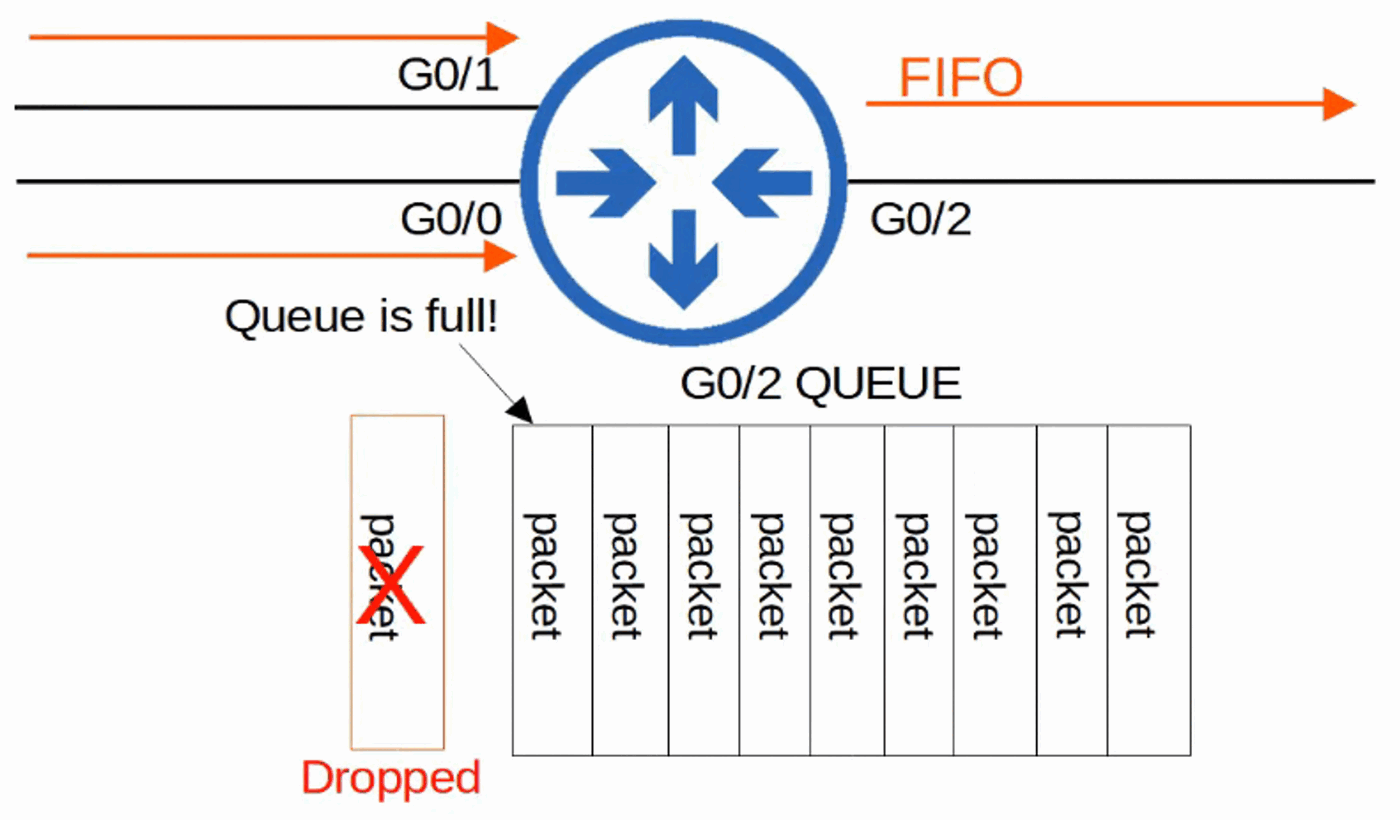
\includegraphics[keepaspectratio,alt={image}]{images/48-qos-quality-of-service/img-021.png}}
\end{figure}

\begin{itemize}
\tightlist
\item
  An essential part of QoS is the use of MULTIPLE QUEUES

  \begin{itemize}
  \tightlist
  \item
    This is where CLASSIFICATION plays a role.
  \item
    DEVICE can match TRAFFIC based on various factors (like DSCP
    MARKINGS in the IP HEADER) and then place it in the appropriate
    QUEUE
  \end{itemize}
\item
  HOWEVER, the DEVICE is only able to forward one FRAME out of an
  INTERFACE at once SO a \emph{SCHEDULER}, is used to decide which QUEUE
  TRAFFIC is FORWARDED from the next

  \begin{itemize}
  \tightlist
  \item
    \emph{PRIORITZATION} allows the SCHEDULER to give certain QUEUES
    more PRIORITY than others
  \end{itemize}
\end{itemize}

\begin{figure}
\centering
\pandocbounded{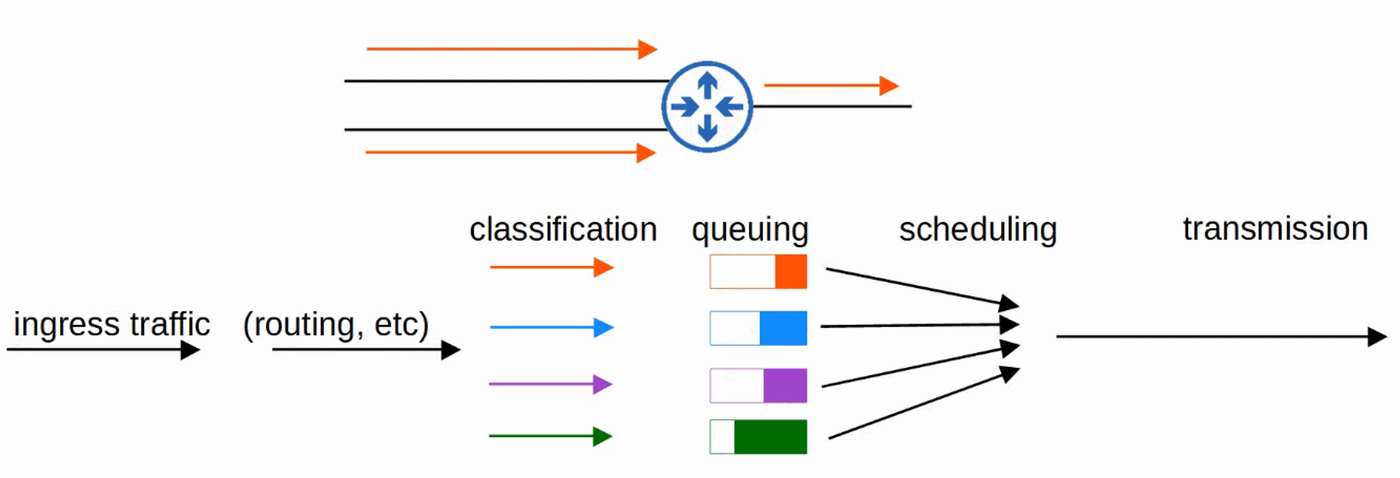
\includegraphics[keepaspectratio,alt={image}]{images/48-qos-quality-of-service/img-022.png}}
\end{figure}

\begin{itemize}
\tightlist
\item
  A COMMON scheduling method is \emph{WEIGHTED ROUND-ROBIN}

  \begin{itemize}
  \tightlist
  \item
    ROUND-ROBIN:

    \begin{itemize}
    \tightlist
    \item
      PACKETS taken from each QUEUE in order, cyclically
    \end{itemize}
  \item
    WEIGHTED:

    \begin{itemize}
    \tightlist
    \item
      More DATA taken from HIGH PRORITY QUEUES each time the SCHEDULER
      reaches that QUEUE
    \end{itemize}
  \end{itemize}
\item
  CBWFQ (CLASS BASED WEIGHED FAIR QUEUING)

  \begin{itemize}
  \tightlist
  \item
    Popular method of SCHEDULING
  \item
    Uses WEIGHTED ROUND-ROBIN SCHEDULER while guaranteeing each QUEUE a
    certain PERCENTAGE of the INTERFACE'S bandwidth during CONGESTION
  \end{itemize}
\end{itemize}

\begin{figure}
\centering
\pandocbounded{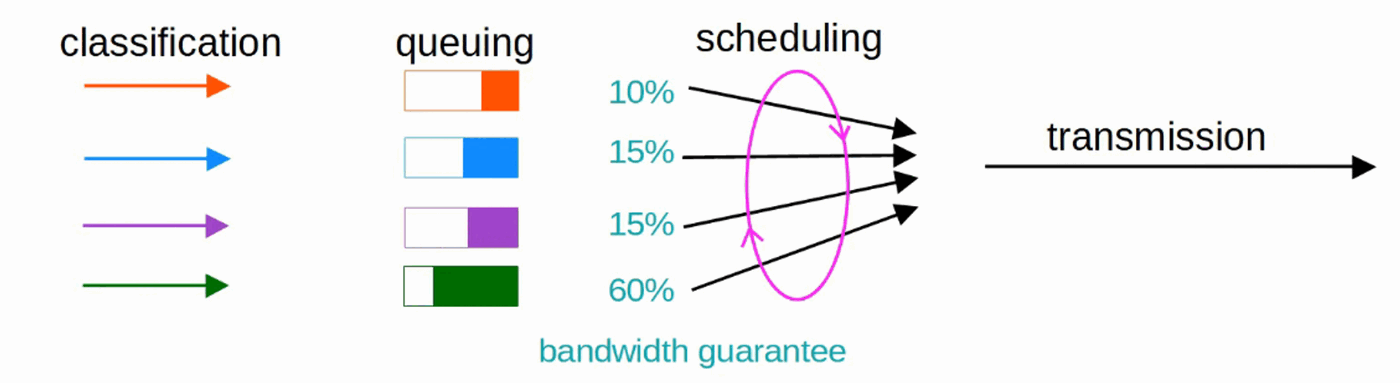
\includegraphics[keepaspectratio,alt={image}]{images/48-qos-quality-of-service/img-023.png}}
\end{figure}

\begin{itemize}
\tightlist
\item
  ROUND-ROBIN SCHEDULING is NOT IDEAL for VOICE / VIDEO TRAFFIC

  \begin{itemize}
  \tightlist
  \item
    Even if VOICE / VIDEO TRAFFIC receives a guaranteed MINIMUM amount
    of BANDWIDTH, ROUND-ROBIN can add DELAY and JITTER because even the
    HIGH PRIORITY QUEUES have to wait their turn in the SCHEDULER
  \end{itemize}
\item
  LLQ (LOW LATENCY QUEUING)

  \begin{itemize}
  \tightlist
  \item
    Designates ONE (or more) QUEUES as \emph{strict priority queues}
  \item
    This means that if there is TRAFFIC in the QUEUE, the SCHEDULER will
    ALWAYS take the next PACKET from that QUEUE until it is EMPTY
  \item
    This is VERY EFFECTIVE for reducing the DELAY and JITTER of VOICE /
    VIDEO TRAFFIC
  \item
    HOWEVER, LLQ has a DOWNSIDE of potentially starving other QUEUES if
    there is always TRAFFIC in the DESIGNATED \emph{STRICT PRIORITY
    QUEUE}

    \begin{itemize}
    \tightlist
    \item
      POLICING can control the AMOUNT of TRAFFIC allowed in the
      \emph{STRICT PRIORITY QUEUE} so that it can't take all of the
      link's BANDWIDTH
    \end{itemize}
  \end{itemize}
\end{itemize}

\begin{figure}
\centering
\pandocbounded{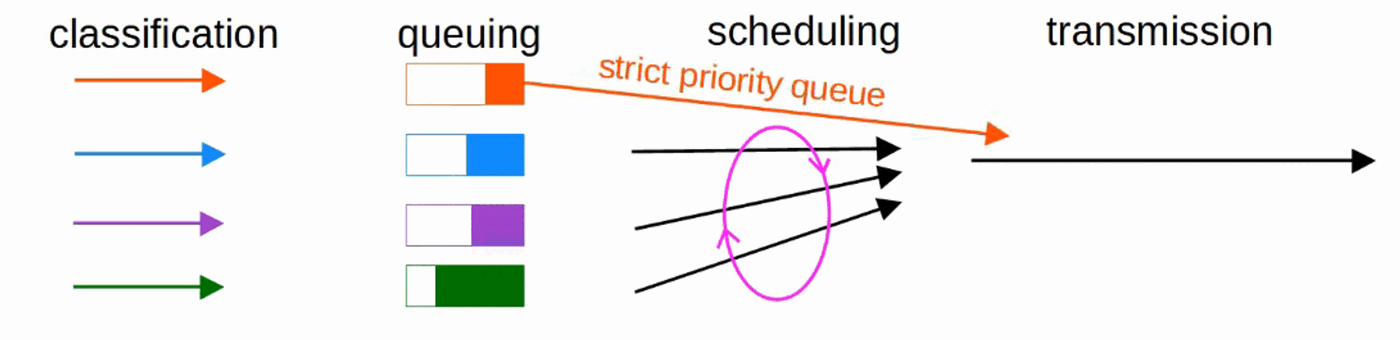
\includegraphics[keepaspectratio,alt={image}]{images/48-qos-quality-of-service/img-024.png}}
\end{figure}

\section{Shaping / Policing}\label{shaping-policing}

\begin{itemize}
\tightlist
\item
  TRAFFIC SHAPING and POLICING are both used to control the RATE of
  TRAFFIC
\item
  SHAPING

  \begin{itemize}
  \tightlist
  \item
    Buffers TRAFFIC in a QUEUE if the TRAFFIC RATE goes over the
    CONFIGURED RATE
  \end{itemize}
\item
  POLICING

  \begin{itemize}
  \tightlist
  \item
    DROPS TRAFFIC if the TRAFFIC RATE goes over the CONFIGURED RATE

    \begin{itemize}
    \tightlist
    \item
      POLICING also has the option of RE-MARKING the TRAFFIC, instead of
      DROPPING
    \end{itemize}
  \item
    ``BURST'' TRAFFIC over the CONFIGURED RATE is allowed for a short
    period of time
  \item
    This accommodates DATA APPLICATIONS which typically are ``bursty''
    in nature (ie: not constant stream)
  \item
    The amount of BURST TRAFFIC allowed is configurable
  \end{itemize}
\item
  In BOTH cases, CLASSIFICATION can be used to ALLOW for different RATES
  for different KINDS of TRAFFIC
\item
  WHY would you want to LIMIT the RATE that TRAFFIC is SENT / RECEIVED ?
\end{itemize}

\begin{figure}
\centering
\pandocbounded{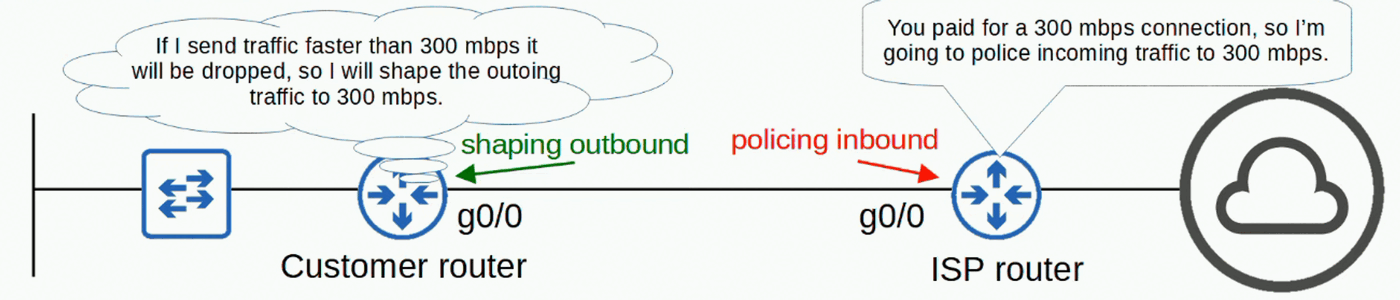
\includegraphics[keepaspectratio,alt={image}]{images/48-qos-quality-of-service/img-025.png}}
\end{figure}
